\begin{figure}[h]
    \begin{subfigure}[t]{\columnwidth}
        \centering
        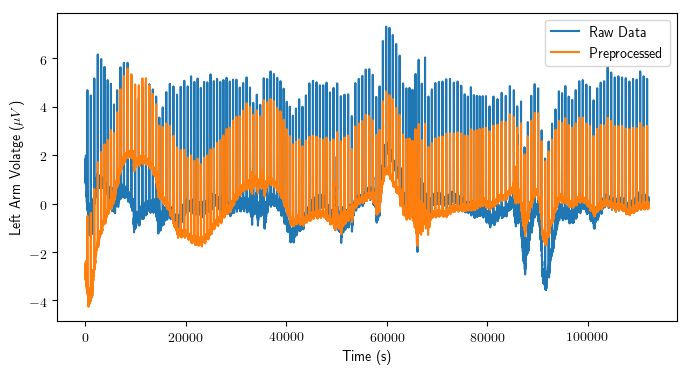
\includegraphics[width=\columnwidth]{tex/figures/filtering/ECG Left Arm time.png}
        \caption{Left}
        \label{fig:filter:left:time}
    \end{subfigure}
    \begin{subfigure}[t]{\columnwidth}
        \centering
        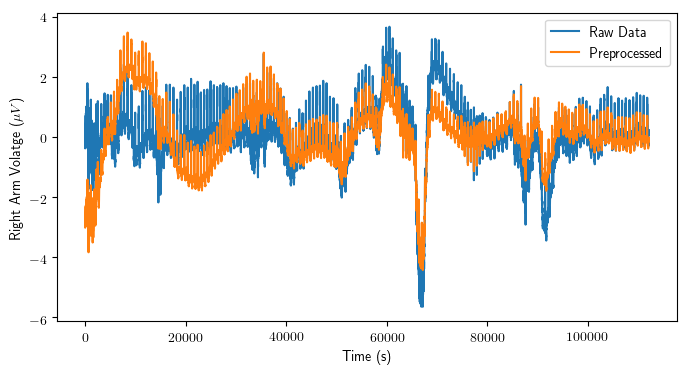
\includegraphics[width=\columnwidth]{tex/figures/filtering/ECG Right Arm time.png}
        \caption{Right}
        \label{fig:filter:right:time}
    \end{subfigure}
    \caption{Example filtering of ECG signal on sample 1 video 12
             for the left and right arms in time domain}
    \label{fig:ecg:time}
\end{figure}
\begin{figure}[h]
    \centering
    \begin{subfigure}[t]{\columnwidth}
        \centering
        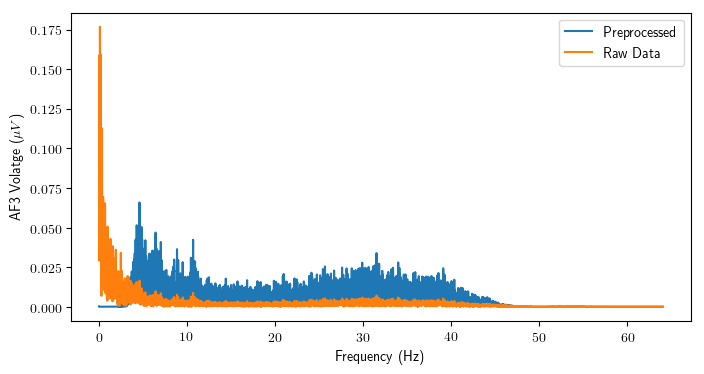
\includegraphics[width=\columnwidth]{tex/figures/filtering/AF3.png}
        \caption{AF3}
        \label{fig:filter:af3}
    \end{subfigure}
    \caption{Example filtering of EEG signal on sample 1 video 12}
    \label{fig:eeg}
\end{figure}
\begin{figure}[h]
    \begin{subfigure}[t]{\columnwidth}
        \centering
        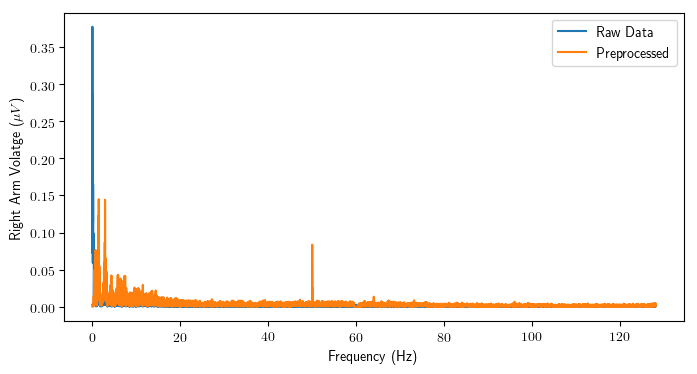
\includegraphics[width=\columnwidth]{tex/figures/filtering/ECG Right Arm.png}
        \caption{Right}
        \label{fig:filter:right}
    \end{subfigure}
    \caption{Example filtering of ECG signal on sample 1 video 12
             for the left and right arms}
    \label{fig:ecg}
\end{figure}
